%\chapter{Moyens d'identification généralement utilisés}
\chapter{Moyens d'identification}
\section{Imperfections du principe de même origine}
La possibilité de violer le principe de même origine est la source de nombreuses méthodes qui permettent de tracer les utilisateurs.
En effet, elle permet à un site A de créer et récupérer un cookie sur l'ordinateur de l'utilisateur s'il visite un autre site B qui inclut du contenu du site A (\autoref{cookies}). Cela autorise également des sites à accéder à des éléments d'un autre site enregistrés en cache (\autoref{cache}).

L'absence d'implémentation du principe de même origine dans l'historique de l'utilisateur permet de déterminer si le navigateur a été utilisé pour visiter un site en regardant la couleur des liens hypertextes pointant vers ce site. Dans ce cas, l'utilisation de cookies n'est même plus nécessaire.
\newline

Le traçage des utilisateurs peut être classé en plusieurs catégories \cite{Jackson:2006:PBS:1135777.1135884} :
\begin{itemize}
  \item tracking sur une seule session : inévitable vu comment le Web fonctionne
  \item tracking sur de multiples sessions : permet à un site d'identifier un visiteur s'il revient plus tard sur le site
  \item tracking coopératif : permet à des sites coopérants de créer un historique des visites d'un utilisateur sur tous les sites de la coopération
  \item tracking semi-coopératif sur un seul site : permet à un site de déterminer des informations sur les activités d'un visiteur sur un autre site en y plaçant du contenu (par exemple, en plaçant une image sur un forum)
  \item tracking semi-coopératif sur de multiples sites : identique au tracking semi-coopératif sur un seul site à l'exception qu'il peut y avoir plusieurs sites ciblés
  \item tracking non coopératif : permet à un site de déterminer des informations sur les activités d'un visiteur sur un autre site sans participation du site ciblé
  \newline
\end{itemize}

Certains types de tracking peuvent être évités en améliorant le principe de même origine mais il est malheureusement difficile de contrer les types de tracking dits coopératifs.

%%%%%%%%%%%%%%%%%%%%%%%%%%%%%%
\section{Cookies}
\label{cookies}
En ce qui concerne les cookies, il est assez simple de tracer la navigation d'un utilisateur. En effet, nous avons vu que le navigateur envoie dans chaque requête HTTP un en-tête \textit{Cookie}. Il est donc aisé pour le site web de suivre le parcours du visiteur simplement en analysant cet en-tête. Le fait de passer par un proxy ne change rien car le cookie reste indépendant du moyen d'accès au site web.
\newline

En général, on utilise deux types de classification pour les cookies \cite{Yue:2007:ACU:1251984.1253093}.

Le premier se base sur l'origine et la destination : les cookies sont classifiés en tant que cookies "first-party" ou "third-party". Les cookies "first-party" sont issus du domaine que l'utilisateur est en train de visiter, on les appelle cookies d'origine ou cookies de domaine. Les cookies "third-party" sont créés par un site autre que celui qui est visité par l'utilisateur, on les appelle cookies tiers.

La seconde méthode de classification se base sur la durée de vie du cookie : les cookies sont alors classifiés en cookies de session ou cookies persistants. Les cookies de session sont stockés dans la mémoire vive de l'ordinateur et supprimés à la fermeture du navigateur. A l'opposé, les cookies persistants sont stockés sur le disque dur de l'ordinateur et supprimés soit lors de leur expiration, soit manuellement par l'utilisateur.
\newline

Les cookies tiers, qu'ils soient de session ou persistants, n'apportent quasiment aucun bénéfice à l'utilisateur. Ils sont d'ailleurs reconnus comme une menace pour la vie privée et les navigateurs proposent généralement une option pour les désactiver.

Les cookies d'origine de type session ne posent pas vraiment de problèmes relatifs à la vie privée étant donné leur faible durée de vie.

A l'opposé, les cookies d'origine persistants peuvent poser des problèmes divers. En effet, les cookies persistants sont une arme à double tranchant : ils peuvent jouer un rôle utile en permettant la personnalisation et l'authentification sur les sites mais ils peuvent également jouer un rôle plus dangereux qui amène des risques au niveau de la vie privée et de la sécurité. Ces risques reposent sur deux aspects : le premier, et celui qui nous intéresse principalement ici, est que les cookies persistants permettent de tracer l'activité de l'utilisateur. Le deuxième risque est qu'ils peuvent être volés ou manipulés par des attaques de deux types : les attaques XSS (elles exploitent les vulnérabilités des applications Web) et les attaques qui exploitent les vulnérabilités des navigateurs Web (via notamment le contournement du principe de même origine).
\newline

Une étude menée sur plus de 5000 sites à propos de l'utilisation des cookies \cite{Yue:2007:ACU:1251984.1253093} a montré que les cookies d'origine persistants sont largement utilisés et que plus de 60\% sont réglés pour expirer plus d'un an après leur création.
\newline

Désactiver tous les cookies tiers et garder les cookies d'origine de type session est supporté par la majorité des navigateurs actuels. Le problème se situe au niveau des cookies d'origine persistants car on ne sait pas comment les gérer et déterminer s'ils sont utiles ou néfastes pour l'utilisateur.

%- parler des cookies de cache dans la section cookies ou dans la section cache ?

%%%%%%%%%%%%%%%%%%%%%%%%%%%%%%
\section{Cache}
\label{cache}
Le cache du navigateur permet d'enregistrer localement une copie des fichiers afin de ne pas devoir les recharger lors d'une visite ultérieure. Ce mécanisme est très utile car il permet d'économiser de la bande passante et du temps. Cependant, il donne la possibilité à des sites web de déterminer si leurs visiteurs ont visité un autre site auparavant.

L'exploitation du cache à des fins de surveillance est détaillé par Felten et Schneider \cite{Felten:2000:TAW:352600.352606}.
Le principe est assez simple : il exploite le fait qu'un fichier présent en cache sera chargé beaucoup plus rapidement qu'un fichier qui ne l'est pas. Donc en mesurant le temps d'accès au fichier, il est possible de déterminer si une personne a déjà visité le site web (ou plus précisément, la page) qui utilise ce fichier. En effet, rien n'empêche un site web de charger un fichier hébergé par un autre site.
\newline

Imaginons que l'administrateur d'un site \emph{(alpha.com)} veuille savoir si ses visiteurs se sont également rendus sur un autre site \emph{(beta.com)}. La première chose qu'il doit faire est de se rendre sur le site qu'il veut cibler et choisir un fichier statique pouvant être mis en cache et qui est chargé par tout visiteur (un logo par exemple). Ensuite, le but est de mesurer le temps d'accès du fichier cible.

Le plus fiable et facile est d'utiliser un applet Java ou un JavaScript qui va mesurer le temps de chargement du fichier à partir de son URL. Même si l'utilisateur a désactivé l'exécution de Java et de JavaScript, il est possible d'obtenir une mesure suffisamment précise en chargeant les fichiers suivants dans l'ordre :

\begin{enumerate}
  \item un fichier du site \emph{alpha.com}
  \item le fichier cible du site \emph{beta.com}
  \item un autre fichier du site \emph{alpha.com}
\end{enumerate}

En soustrayant les moments auxquels le serveur reçoit les requêtes des fichiers 1 et 3, l'administrateur du site \emph{alpha.com} est en mesure d'avoir une approximation du temps qu'il a fallu pour charger le fichier 2 (celui de \emph{beta.com}).

Il faut néanmoins respecter certains critères pour que cela fonctionne : forcer le chargement des fichiers de manière séquentielle et de manière invisible en n'altérant pas l'apparence de la page afin que le client ne remarque rien.
\newline

Il est possible d'améliorer la probabilité de distinguer correctement les succès des défauts de cache en effectuant différentes mesures, ce qui permet alors de raffiner les seuils de discrimination : refaire plusieurs fois la mesure d'un même fichier (à partir de la seconde tentative, le fichier sera présent dans le cache) pour les succès de cache et utiliser l'URL de fichiers n'existant pas pour les défauts de cache.

Afin d'améliorer la précision, il est également intéressant de combiner les résultats de plusieurs fichiers mesurés individuellement.
\newline

D'une manière semblable, ce type d'attaque peut également être réalisé sur le cache du DNS. Felten et Schneider ont vérifié la précision des tests avec l'aide de 3 serveurs distincts situés à des distances différentes.

Plus le serveur est situé à une grande distance, plus la requête DNS prend de temps. Les tests ont montré que la précision des résultats pouvait être inférieure car la pénalité suite à des défauts de cache était très petite. Il n'était donc pas possible de discriminer les échecs des succès de cache. Cependant, sur Internet, la pénalité en cas de défaut est suffisamment grande pour assurer une bonne distinction. Dans ce cas-là, les tests montrent une très bonne précision.
\newline

% Attache de cookies de cache

Cette attaque peut être menée dans différentes situations :
\begin{itemize}
  \item Un site web qui veut en savoir davantage sur ses visiteurs.
  \item Une régie publicitaire pourrait inclure le code de mesure dans les bannières qu'elle distribue afin de faire des statistiques sur les sites web consultés par les visiteurs.\\Il est même possible de distribuer un code différent pour les catégoriser.
  \item L'attaquant pourrait créer un site web de telle façon à ce qu'il apparaisse en tête des moteurs de recherche dans le but de faire des statistiques sur les personnes intéressées par un sujet particulier.
  \item L'attaquant pourrait envoyer un mail contenant le code HTML à sa victime.\\En le faisant ressembler à du spam, la victime ne remarquerait rien d'anormal et la mesure serait effectuée.
\end{itemize}

% Timing Attacks on Web Privacy (section 1) : raisons de s'inquiéter
% Timing Attacks on Web Privacy (section 7) : contre-mesures actuelles sont inefficaces
% Timing Attacks on Web Privacy (section 8) : solution possible


%%%%%%%%%%%%%%%%%%%%%%%%%%%%%%
\section{Pixels espions}
Les pixels espions sont des images de taille minime (généralement, de 1 pixel de haut sur 1 pixel de large) et sont destinés à effectuer une requête HTTP vers un serveur sans que le visiteur de la page ne s'en aperçoive. L'administrateur du site hébergeant ce pixel espion peut dès lors analyser les logs de son serveur Web afin d'obtenir des informations sur l'utilisateur. En plaçant un pixel espion spécifique sur chaque site, l'administrateur peut distinguer sans problème les requêtes provenant des différents sites et ainsi déterminer quel site a été visité par chaque utilisateur. De plus, en analysant la requête, il peut connaître l'heure à laquelle le visiteur s'est rendu sur la page mais également d'autres informations telles que le navigateur utilisé, le système d'exploitation, etc.

%%%%%%%%%%%%%%%%%%%%%%%%%%%%%%
\section{JavaScript}
JavaScript permet d'exécuter des scripts du côté client. Il a entraîné le déploiement d'applications riches et accessibles simplement via un navigateur Web. Les possibilités sont multiples : il est ainsi facile de se divertir grâce à un jeu écrit en JavaScript mais il est également aisé d'en savoir plus sur l'utilisateur via le navigateur qui exécute le script. Ceci est possible grâce à l'accès dont dispose JavaScript sur l'ordinateur du client. En effet, différents attaques peuvent être perpétrées avec JavaScript afin d'identifier les utilisateurs \cite{Jang:2010:ESP:1866307.1866339}.
\newline

\begin{itemize}
	\item Le vol de cookies : le script inclus depuis un site tiers a accès à toutes les informations présentes sur la page. Lorsque celle-ci fait appel à un script, elle lui donne accès aux cookies, à la barre d'adresses et à l'ensemble des éléments disponibles sur la page. Le script a donc la capacité de lire le contenu des cookies associés au site et de l'envoyer à un site tiers (une régie publicitaire par exemple).
	\item Le détournement d'adresse : le script, ayant l'accès complet au contenu de la page, peut influencer les valeurs des URL. Le script peut également rediriger le navigateur vers un autre site et le rediriger ensuite vers le site d'origine sans que l'utilisateur ne s'en aperçoive (au chargement de la page par exemple).
	\item L'analyse de l'historique : l'attaque consiste à regarder comment les liens sont affichés par le navigateur. En effet, s'ils ont été visités, les liens s'affichent d'une autre couleur. Il suffit alors de créer un lien vers le site que l'on désire cibler dans une partie invisible de la page et utiliser l'interface DOM du navigateur pour regarder comment celui-ci affiche le lien. Cette attaque est possible car dans la plupart des navigateurs, l'accès à un historique de pages visitées, de fichiers cachés et de cache DNS est partagé entre les domaines.
	\item Le traçage de comportement : il est possible de déterminer avec précision le comportement de l'utilisateur sur la page qu'il visite. L'élaboration d'une ligne du temps avec les interactions de l'utilisateur (clics, mouvements, défilements, parties de texte surlignées,...) est réalisable avec l'aide de gestionnaires d'événements. Cet ensemble d'interactions peut alors être envoyé à un site tiers afin de calculer des statistiques sur la navigation de l'utilisateur.
\end{itemize}

\subsection{Régies publicitaires sur Internet}

\subsection{Modules des réseaux sociaux}
Les réseaux sociaux proposent généralement de placer un plugin social qui permet aux visiteurs d'un site d'interagir et de partager avec leurs amis. Bien sûr, l'intégration d'un tel script permet aux plateformes de réseaux sociaux de suivre la navigation des visiteurs d'un site. Si beaucoup de sites intègrent ces scripts, les réseaux sociaux sont alors en mesure d'obtenir une sorte de carte d'Internet avec les déplacements et actions de chaque utilisateur. De plus, si un visiteur est connecté à son compte sur un réseau social en naviguant sur d'autres sites, la plateforme peut directement faire le lien entre son profil et les sites qu'il visite.

\subsubsection{Facebook}
Le code que les gestionnaires de sites Web doivent intégrer au sein de leur page afin d'accéder aux fonctionnalités offertes par Facebook \cite{javascript_facebook_sdk} est visible à la \autoref{js_facebook_sdk}.

\begin{figure}[h]
	\centering
	\lstinputlisting{examples/js_facebook_sdk}
	\caption{\label{js_facebook_sdk}Le SDK de \textit{Facebook} pour JavaScript}.
\end{figure}

\subsubsection{Google+}
De son côté, Google propose différents scripts à ajouter en fonction des fonctionnalités que le gestionnaire de site Web veut intégrer au sein de sa page (voir \autoref{js_google_plus}). Google propose même de charger de façon asynchrone son script afin d'obtenir des performances optimales (voir \autoref{js_google_plus_async}) \cite{javascript_google_plus}.

\begin{figure}[h]
	\centering
	\lstinputlisting{examples/js_google_plus}
	\caption{\label{js_google_plus}L'API JavaScript de \textit{Google+}}.
\end{figure}

\begin{figure}[h]
	\centering
	\lstinputlisting{examples/js_google_plus_async}
	\caption{\label{js_google_plus_async}L'API JavaScript de \textit{Google+} pour un chargement asynchrone}.
\end{figure}

\subsubsection{LinkedIn}
LinkedIn propose également une API pour connecter les sites avec sa plateforme \cite{javascript_linkedin}. Dans la \autoref{js_linkedin}, on peut même voir que le nom de l'utilisateur (s'il est connecté sur la plateforme) est affiché sur le site. Cet aspect semblera convivial à la majorité des utilisateurs mais cela permet surtout de mieux les suivre lors de leur navigation sur les sites intégrant ce module social.

\begin{figure}[h]
	\centering
	\lstinputlisting{examples/js_linkedin}
	\caption{\label{js_linkedin}L'API JavaScript de \textit{LinkedIn}}.
\end{figure}

\subsection{Outils destinés aux webmasters}
Certaines plateformes proposent aux gestionnaires de sites Web de suivre la navigation des visiteurs sur leur site. Elles regardent d'où viennent les visites (moteur de recherche, accès direct, lien d'un autre site,...), leur navigateur (la version, les plugins installés, la langue,...), sur quels pages les visiteurs se rendent, combien de temps ils restent sur chaque page, etc.

\subsubsection{Google Analytics (Universal Analytics)}
\label{google_analytics}
Une des principales plateformes de suivi des utilisateurs est Google Analytics. Cet outil est utilisé par de nombreux gestionnaires de sites afin de connaître les statistiques de fréquentation de leur site \cite{javascript_google_analytics}.

Comme on peut le voir sur la \autoref{Google_Analytics_1}, les statistiques sont très détaillées. Dans la \autoref{Google_Analytics_2}, la ville des visiteurs était affichée mais il est également possible de voir d'autres données telles que leur FAI ou leur système d'exploitation. Des données spécifiques aux clients mobiles sont également disponibles. Toutes les données sont affichées dans des graphiques clairs et dynamiques et il est même possible d'exporter l'ensemble de ces données dans différents formats (CSV, TSV, Excel, PDF,...) afin de les traiter de manière automatique.
\newline

Google a developpé une nouvelle version de son outil d'analyse des visiteurs : Universal Analytics. Ce nouvel outil repose sur le même socle que Google Analytics mais il apporte de nouvelles fonctionnalités.

Pour ce nouvel outil, Google propose 3 types de code de tracking en fonction des plateformes visées : la librairie JavaScript \textit{analytics.js} pour les sites Web, les SDK Google Analytics pour les applications mobiles et le \textit{protocole de mesure ("Measurement Protocol")} pour les autres appareils tels que consoles de jeux et les kiosques d'information.
\newline

Alors que Google Analytics identifiait un utilisateur différent en fonction de chaque appareil connecté, Universal Analytics reconnaît un même utilisateur qui utilise plusieurs moyens de se connecter à Internet. Afin d'y parvenir, ils utilisent un identifiant d'utilisateur unique afin d'associer les données reçues d'appareils et de sessions différentes.

Afin d'utiliser cette fonctionnalité, les gestionnaires de sites Web doivent être en mesure de générer un identifiant unique pour chaque utilisateur et l'associer aux données envoyées à Google. Généralement, cet identifiant unique est généré grâce à l'authentification des visiteurs sur un site. Ainsi, lorsqu'un utilisateur se sert de sa tablette et de son ordinateur pour se rendre sur un site et s'il s'y connecte, Google sera en mesure d'identifier ces visites comme provenant d'un seul et même utilisateur et non plus de deux utilisateurs différents.
\newline

En fonction de la version de Google Analytics utilisée, différents cookies sont créés et utilisés afin de suivre les visites des utilisateurs \cite{Google_Analytics_cookies}.
\newline

La nouvelle librairie JavaScript de Google, \textit{analytics.js} crée un cookie d'origine contenant un identifiant anonyme afin de distinguer les utilisateurs. Par défaut, la librairie crée un cookie sur le domaine de plus haut niveau et règle le chemin du cookie sur le niveau racine.

Le cookie créé est :
\begin{itemize}
  \item \textbf{\_ga} : cookie avec une date d'expiration de 2 ans destiné à distinguer les utilisateurs.
  \newline
\end{itemize}

L'ancienne libraire JavaScript de Google, \textit{ga.js}, crée 5 cookies d'origine qui permettent de :
\begin{itemize}
  \item déterminer quel domaine est mesuré
  \item distinguer les utilisateurs uniques
  \item se souvenir du nombre et des heures des visites précédentes
  \item se souvenir de l'information sur la source de trafic
  \item déterminer le début et la fin de session
  \item se souvenir des valeurs des variables personnalisées au niveau de l'utilisateur
\end{itemize}

Par défaut, la librairie crée un cookie sur le domaine spécifié dans la propriété du navigateur \textit{document.host} et règle le chemin du cookie sur le niveau racine.

Les cookies créés sont:
\begin{itemize}
  \item \textbf{\_\_utma} : cookie avec une date d'expiration de 2 ans destiné à distinguer les utilisateurs et les sessions.
  \item \textbf{\_\_utmb} : cookie avec une date d'expiration de 30 minutes destiné à distinguer les nouvelles sessions et visites.
  \item \textbf{\_\_utmc} : cookie avec une date d'expiration de fin de session qui n'est plus utilisé dans \textit{ga.js} mais qui permet l'interopérabilité avec \textit{urchin.js} (une librairie encore plus ancienne de Google Analytics, antérieure à \textit{ga.js}).
  \item \textbf{\_\_utmz} : cookie avec une date d'expiration de 6 mois destiné à enregistrer les sources de trafic ou de campagne qui explique comment un utilisateur atteint le site.
  \item \textbf{\_\_utmv} : cookie avec une date d'expiration de 2 ans utilisé pour sauvegarder les données des variables personnalisées au niveau de l'utilisateur.
\end{itemize}

\begin{figure}[h]
	\centering
	\lstinputlisting{examples/js_google_analytics}
	\caption{\label{js_google_analytics}L'API JavaScript de \textit{Google Analytics}}.
\end{figure}

\begin{figure}[h]
	\centering
	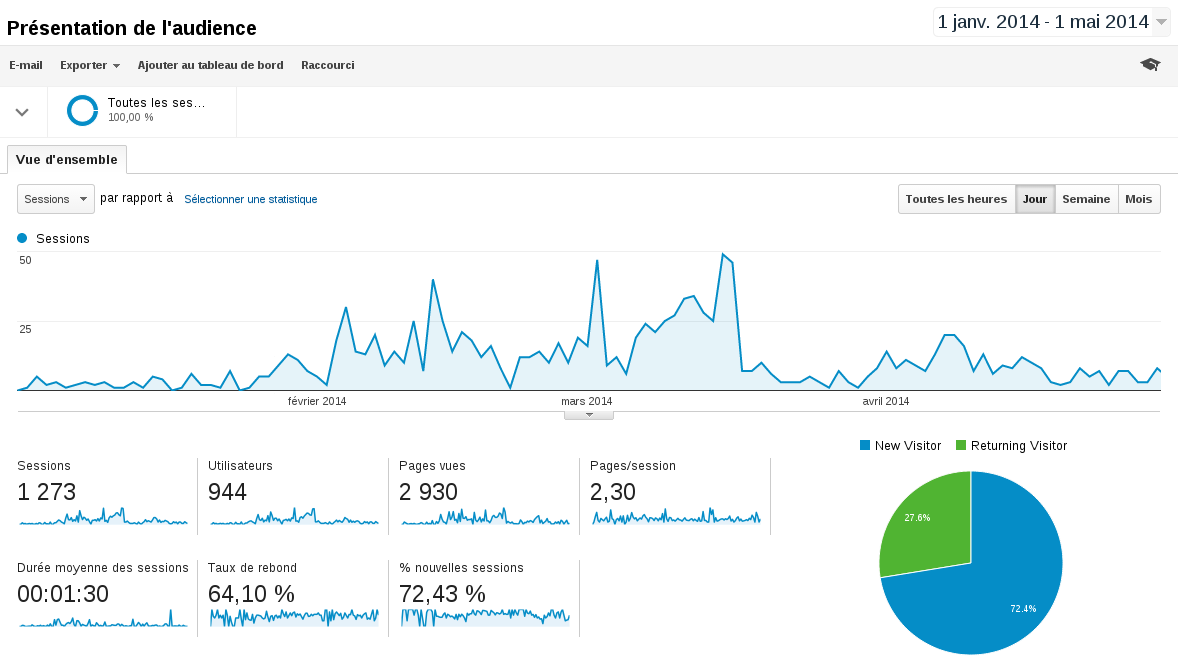
\includegraphics[scale=0.4]{examples/Google_Analytics_1.png}
	\caption{\label{Google_Analytics_1}Copie d'écran de \textit{Google Analytics} qui détaille la navigation sur le site}
\end{figure}

\begin{figure}[h]
	\centering
	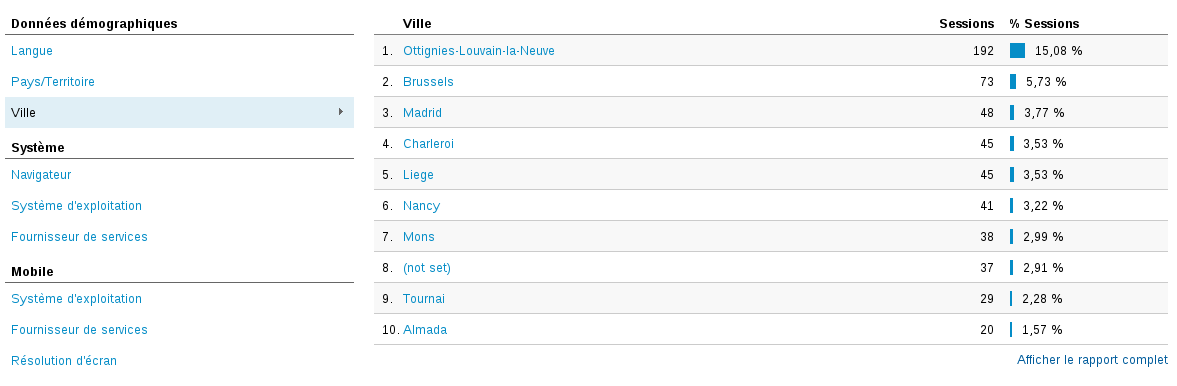
\includegraphics[scale=0.4]{examples/Google_Analytics_2.png}
	\caption{\label{Google_Analytics_2}Copie d'écran de \textit{Google Analytics} qui détaille l'origine des visiteurs}
\end{figure}

%%%%%%%%%%%%%%%%%%%%%%%%%%%%%%
\section{Flash}



%%%%%%%%%%%%%%%%%%%%%%%%%%%%%%
\section{Empreintes des navigateurs}
\label{fingerprinters}
